%% Template for Memo Series
%% Please modify the MEMO-data section below and
%% paste the report text into the space at the end of this file.
\documentclass[british]{article}
\usepackage{mathptmx}
\usepackage[T1]{fontenc}
\usepackage[latin9]{inputenc}
\usepackage[letterpaper]{geometry}
\geometry{verbose,tmargin=3cm,bmargin=3cm,lmargin=3cm,rmargin=3cm}
\usepackage{fancyhdr}
\pagestyle{fancy}
\usepackage{graphicx}
\usepackage{setspace}
\usepackage{subfigure}
%\usepackage{subcaption}
\onehalfspacing

% Extra packages
\usepackage{algpseudocode}
\usepackage{algorithm}
\usepackage{booktabs}
\usepackage{cleveref}
\usepackage{amssymb}

\makeatletter

%%%%%%%%%%%%%%%%%%%%%%%%%%%%%% LyX specific LaTeX commands.
\newcommand{\lyxline}[1][1pt]{%
  \par\noindent%
  \rule[.5ex]{\linewidth}{#1}\par}

\newcommand{\noun}[1]{\textsc{#1}}

\makeatother

\usepackage{babel}
\begin{document}
%% MEMO-data section to define report name, authors, contacts, date, number, etc.
%% Please modify it as appropriate.
\def\MEMOtitle{Automated translation of concepts to Finite State Machines}
\def\MEMOauthors{Jonathan Beaumont, Adrian Wheeldon}
\def\MEMOcontacts{\{j.r.beaumont, a.r.wheeldon2\}@ncl.ac.uk}
\def\MEMOyear{2017}
\def\MEMOdate{March \MEMOyear}
\def\MEMOnumber{NCL-EEE-MICRO-MEMO-\MEMOyear-010}
%% End od MEMO-data section

%% Page decoration options for the body of the memo
\pagenumbering{arabic}
\renewcommand{\headrulewidth}{0.4pt}
\renewcommand{\footrulewidth}{0.4pt}
\lhead{\MEMOauthors: \MEMOtitle}
\chead{}
\rhead{}
\lfoot{\MEMOnumber, Newcastle University}
\cfoot{}
\rfoot{\thepage}
\sloppy

\thispagestyle{empty}

\begin{center}
{\Large ~}{\footnotesize \vspace{-22mm}
}
\par\end{center}{\footnotesize \par}

{\Large \lyxline{\Large}}{\Large \par}

\begin{center}
%
\begin{minipage}[b][1\totalheight][t]{0.45\columnwidth}%
{\footnotesize 
\includegraphics[scale=0.14]{logonewcastle.jpg}}{\footnotesize \par}

\noindent {\footnotesize \smallskip{}
}{\footnotesize \par}

{\footnotesize Copyright~\copyright~\MEMOyear~Newcastle University}%
\end{minipage}%
\begin{minipage}[b][1\totalheight][t]{0.45\columnwidth}%
\noindent {\footnotesize $\mu$Systems Research Group}\\
{\footnotesize School of Electrical and Electronic Engineering}\\
{\footnotesize Merz Court}\\
{\footnotesize Newcastle University}\\
{\footnotesize Newcastle upon Tyne, NE1 7RU, UK}{\footnotesize \par}

\noindent {\footnotesize \medskip{}
}{\footnotesize \par}

\noindent \texttt{\footnotesize http://async.org.uk/}%
\end{minipage}
\par\end{center}

\lyxline{\normalsize}

\vspace{15mm}

\begin{center}
\textbf{\huge Automated translation of concepts to\\ Finite State Machines}
\par\end{center}{\huge \par}

\begin{center}
\bigskip{}
{\Large \MEMOauthors}
\par\end{center}{\Large \par}

\begin{center}
\texttt{\small \MEMOcontacts}
\par\end{center}{\small \par}

\begin{center}
\bigskip{}
{\large \MEMOnumber}
\par\end{center}{\large \par}

\begin{center}
{\large \MEMOdate}
\par\end{center}{\large \par}

\vspace{15mm}

%% Plato FSM Translation Tech Memo
%% Abstract
\begin{abstract}
  An abstract.
\end{abstract}

\newpage{}

\thispagestyle{fancy}


% Add sections here
%% Plato FSM Translation Tech Memo
%% Introduction

\section{Introduction \label{sec:intro}}

As discussed in~\cite{2015_Beaumont_MEMOCODE}, concepts are a useful language
for specifying the behaviours of asynchronous circuits,
in the preferred form of the user. This can be as
low-level signal-level concepts, or higher-level gate or
protocol-level concepts. It also allows the definition
of their own concepts, which can be reused within
the same or any other specification that they wish, to
increase the speed of designing a system, and future
systems.

In~\cite{2016_concept_STG_translation}, we introduce an 
algorithm for automatically translating concepts to Signal Transition Graphs (STGs). 
This is aimed at solving problems that can arise with the monolothic approach
for desigining asynchronous circuits with STGs, such as a lack of reusability, and 
poor scalability. 

Since STGs are so commonly used for desinging asynchronous circuits,
there are several tools available, such as \noun{Petrify}~\cite{Cortadella}, \noun{Mpsat}~\cite{khomenko2004detecting}, \noun{Versify}~\cite{i1997formal},
\noun{Workcraft}~\cite{Sokolov-2016-book-Workcraft}\cite{Workcraft_website}, and others, which can automatically verify and synthesize
asynchronous circuits. Automated translation of concepts to STGs therefore allows concept specifications
to be usable with these tools, avoiding the need to develop verification and synthesis tools specifically for 
concepts, which is a timely process. 

Finite State Machines (FSMs) can be used for a wide range of applications, from small scale
to large scale, low-level to high-level system designs. Because of this, they are commonly taught
as a method of designing overall system operation. This means that many designers in industry
are aware of of FSMs, and are more likely to understand them than STGs, which are developed
and primarily used in academia. For this reason, it may be useful when specifying an asynchronous circuit 
using concepts, to be able to view the system as an FSM, and automatic translation will allow this to occur quickly.

However, while viewing the FSM may be useful for a user, STG tools are still the primary methods of 
verifiying and synthesizing asynchronous circuits. The concepts language does not provide any
concepts only for use when translating to either an FSM or an STG specifically, so any concept specification
which translates to one of these will also produce an equivalent model of the alternative formalism, with
no changes to the specification. Each translation algorithm handles the differences in the two formalisms,
producing the correct construcs for that formalism, based on the provided concepts. 

The open-source command-line tool \noun{Plato}~\cite{2017_plato_github}, is authoured in Haskell, and implements the domain-specific language of concepts, 
as well as the algorithms for translating this language to both STGs and FSMs. \noun{Plato} is included as a
back-end tool for \noun{Workcraft}~\cite{Sokolov-2016-book-Workcraft}\cite{Workcraft_website}, where it is integrated to provide
a graphical user interface for authoring and translating concepts. It also includes STG verification and synthesis tools, thus providing
a streamlined interface for designing asynchronous systems from concept specification, to implementation. 

Our contributions are as follows:
\begin{itemize}

\item We discuss Finite State Machines, their uses, their differences from STGs and how concepts can be used to produce FSMs in Section~\ref{sec:fsms}

\item We present the implemented algorithm for translating
concepts to FSMs in Section~\ref{sec:algorithm}.

\item We present a brief example of the design flow in Section~\ref{sec:design-flow}

\end{itemize}
%% Plato FSM Translation Tech Memo
%% FSM background
\newpage
\section {Finite State Machines \label {sec:fsms}}

Finite State Machines can be used to model behaviour of all levels of system~\cite{Taraate2016}. 
The formalism contains states, which are the vertices, and transitions between these states, which 
are the arcs. Applied to each transition is the event for that transition to occur, causing a change 
of state. Depending on the level of system that is being modelled, this event can be a condition being met,
such as the temperature being over a certain value, or it could be a signal transition. 

Regardless of system level, an FSM model always shows some key parts of the system. Each state a system is 
in usually has an associated output or action, which occurs upon entry to this state and continues while the system remains
in this state, and when an event occurs, the state will change depending on what state the system is in, and which event occured. 

For example, Figure~\ref{fig:stopwatch} contains the example FSM which models the 
high-level behaviour of a stopwatch.

\begin{figure}[h]
\begin{centering}
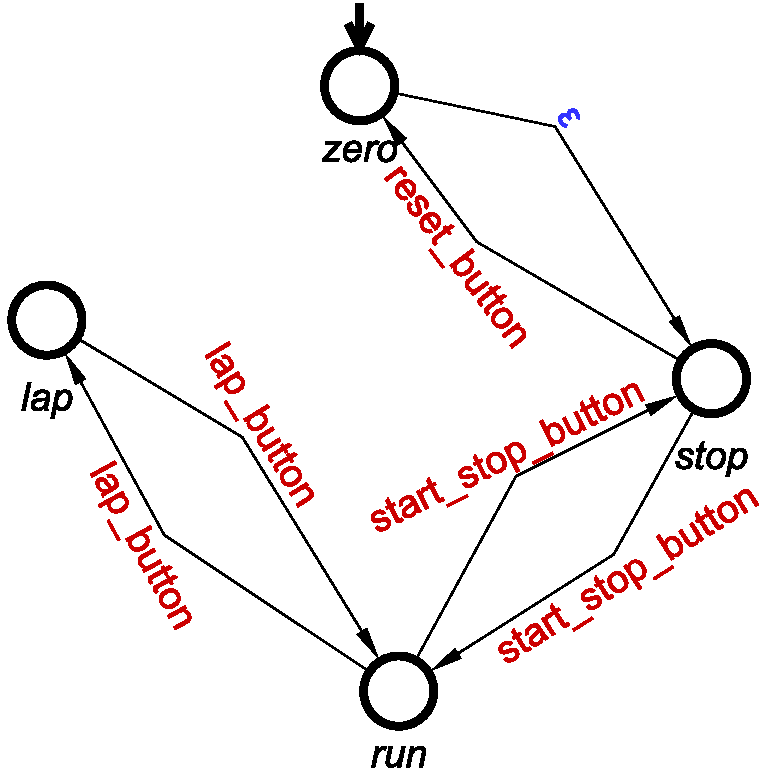
\includegraphics[scale=0.5]{images/stopwatch-fsm}
\par\end{centering}
\protect\caption{\label{fig:stopwatch} Stopwatch FSM}
\end{figure}

\noindent There are four states, which are:

\begin{itemize}

\item Zero - The initial state, where the timer and display are reset to 0. 

\item Stop - In this state, the timer and display are paused.

\item Run - While in this state, the timer is counting, and the display shows this.

\item Lap - In this state, the timer continues counting but the display shows the time when lap was entered.

\end{itemize}

\noindent The transitions between these are based on three buttons:

\begin{itemize} 

\item Reset button - When it has been stopped (in the stop state), moves the system to the zero state to reset everything to 0.

\item Start/Stop button - Used to move the stopwatch from the stop state to the run state, and back. This starts and pauses the timer. 

\item Lap button - This moves the system from the run state, to the lap state, to hold a time on the display for recording. 
                              Also moves it back to the run state, updating the display to the actual time
                              
\end{itemize}

\noindent Also, not that when the zero state is reached, there is an $\varepsilon$ symbol. This symbol represents that
a transition occurs without any requirements. For this example, it is important, as when the system initialises or is reset, we 
want the display and counter to be set to 0, and following this, be ready to start counting. This therefore resets the system, and
moves into the stop state, ready for the timer to being counting from a start/stop button press. 

This is a high-level model as it describes the possible states of the system, but not the low-level implementation details. 
For example, we know what buttons to press to move between states, but there is nothing to say what constitues a button ``press'', 
and, while we know how the display should react depending on the state, we have not provided any details on how we control the display. 

The stopwatch behaviour however does identify the key parts. Each state has an associated action, which we have described. Each transition
has an associated event, these being either button presses, or nothing. We also know that for each state, we can transition to a new state if a
specific button is pressed, but if that button is not associated with a transition from the current state, the state will remain the same, for example, 
if we press the reset button while in the run state, we cannot changes state. 

This example can be used further by adding some implementation details, based on how the components, the buttons and display, work, yet 
the behaviour of the stop-watch will remain the same. 

FSMs can be used to model circuits at the signal-level, as with STGs. In this case, the actions associated with the states can be simply the
arrangement of the signals in the system, the effect of this arrangment causing changes in the environment of the circuit itself. The events 
associated with the transitions between states can be signal transitions. For example, Figure~\ref{fig:handshake-fsm} contains a handshake FSM.

\begin{figure}[h]
\begin{centering}
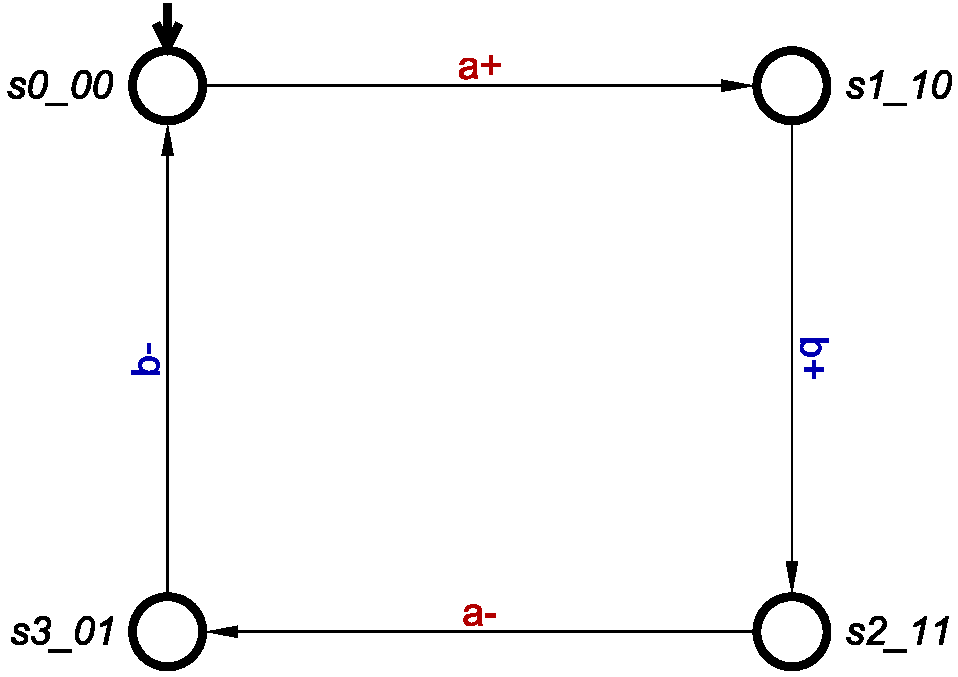
\includegraphics[scale=0.5]{images/handshake-fsm}
\par\end{centering}
\protect\caption{\label{fig:handshake-fsm} Handshake FSM}
\end{figure}

In this example there is one input signal, $a$, one output signal, $b$, and four states: 

\begin{itemize}

\item 00 - The initial state, where both input and output have transitioned low.

\item 10 - The input has gone from 0 to 1.

\item 11 - The output transitions from 0 to 1.

\item 01 - The input transitions low, from 1 to 0.

\end{itemize}

\noindent The transitions between feature the events of these signals transitioning high and low. 

In this case, we have included the implementation details, specifically in what signal transitions cause a changes of state, 
therefore this can be considered a low-level FSM model. However, this doesn't change the fact that the key behaviours are identified. 

Since FSMs can be used generally at all different levels of behavioural modelling, the requirements for what constitutes and event for
a state transition, are not stated, therefore, as with these examples they can be a button press or a signal transition. There exists 
a form of FSM specifically designed for modelling circuit behaviour at signa-level, such as in Figure~\ref{fig:handshake-fsm} named 
\emph{Finite State Transducers} (FSTs). 

FSTs aim to be used for specifications of circuits, and can be used for specifying asynchronous circuits. They allow signals
to be set as specific types, inputs, outputs and internals for example, but do not differ in how they show behaviours. For this reason, 
they can be converted to and from other modelling methods aimed at showing signal-level behaviours such as STGs, and this applies
to \noun{Plato}, where a concept specification must be able to produce either an FSM or an STG without any changes to the specification. 

When using \noun{Workcraft}, an STG can be translated from a concept specification using \noun{Plato} from the STG plugin, and while \noun{Workcraft} does
feature both an FSM and FST plugin, for the interoperability of STGs and FSTs, a concept specification can be translated only to an FST. For this paper however, 
we will continue to FSTs translated from concepts as FSMs. 

\subsection{FSMs and STGs \label{sub:FSMs-STGs}}
%% Plato FSM Translation Tech Memo
%% FSM Translation Algorithm
%%
%% Adrian Wheeldon
%% March 2017
\section{FSM Algorithm}\label{sec:algo}

In order to create a complete encoding of a state, we must first find all of the signals that exist in the system.
We do this by first removing any \emph{effect} transition which may occur in the \emph{cause} list, and then construct a signal list from each causality.
Taking the union of the signal lists from all causalities then gives us the complete set of signals in the system.
In our example, we obtain the list of signals $a$, $b$, $c$.

Now we must add to each causality any signals that are missing so that we can begin to create a complete encoding.
\Cref{tab:enc} shows the new signals in bold, which are added with an `x', or `don't care' polarity since both rising or falling transitions give valid states for these signals.

Now that all signals in the design are accounted for in each causality (that is, the concatenation of \emph{Causes} and \emph{Effect} in \cref{tab:enc} contains all the signals \texttt{a}, \texttt{b}, and \texttt{c}), we can begin constructing state encodings.
We sort the signals such that the binary encoding will represent ascending signal names from left to right -- in this example, \texttt{abc}.
Since the \emph{effect} transition tells us what the effect signal \emph{will become}, we have already obtained the destination state encodings for each arc in the FST\@.
To obtain the source state encodings, we must flip the polarity of the \emph{effect} transition.
The result is shown in \cref{tab:enc}.

Note that we still have `don't care' polarity in some of our state encodings.
Since this means the corresponding signal can be either high or low, we must translate such states into all possible states to obtain a complete FST\@.
We expand these don't care states into all of the possible congruent transition permutations.
For example, from the final row in \cref{tab:enc} we have the states \texttt{x01}, \texttt{x11}.
These will be expanded to the state pairs \texttt{001}, \texttt{011} and \texttt{101}, \texttt{111}.
\Cref{tab:enc_complete} gives the complete source and destination state encodings where the \emph{effect} denotes the FST arc label.

\begin{table}[ht]
\caption{Table}\label{tab:causality}
\centering
\begin{tabular}{@{}ll@{}}
	\toprule
	Causes & Effect\\ \midrule
	$a^{+}$, $b^{+}$	& $c^{+}$ \\
	$a^{-}$, $b^{-}$ 	& $c^{-}$ \\
	$c^{-}$			& $a^{+}$ \\
	$c^{+}$			& $a^{-}$ \\
	$c^{-}$			& $b^{+}$ \\
	$c^{+}$			& $b^{-}$ \\
	\bottomrule
\end{tabular}
\end{table}

\begin{table}[ht]
	\caption{Missing signals added to cause list (bold) with incomplete state encoding.}\label{tab:enc}
\centering
\begin{tabular}{@{}llll@{}}
	\toprule
	& & \multicolumn{2}{c}{Encoding (\texttt{abc})}\\ \cmidrule(l){3-4}
	Causes & Effect & Destination & Source\\ \midrule
	$a^{+}$, $b^{+}$		& $c^{+}$ & \texttt{111} & \texttt{110}\\
	$a^{-}$, $b^{-}$ 		& $c^{-}$ & \texttt{000} & \texttt{001}\\
	$\mathbf{b^{x}}$, $c^{-}$	& $a^{+}$ & \texttt{1x0} & \texttt{0x0}\\
	$\mathbf{b^{x}}$, $c^{+}$	& $a^{-}$ & \texttt{0x1} & \texttt{1x1}\\
	$\mathbf{a^{x}}$, $c^{-}$	& $b^{+}$ & \texttt{x10} & \texttt{x00}\\
	$\mathbf{a^{x}}$, $c^{+}$	& $b^{-}$ & \texttt{x01} & \texttt{x11}\\
	\bottomrule
\end{tabular}
\end{table}

\begin{table}[ht]
\caption{Complete state encodings after expansion of `don't care' states.}\label{tab:enc_complete}
\centering
\begin{tabular}{@{}llll@{}}
	\toprule
	& \multicolumn{2}{c}{Encoding (\texttt{abc})}\\ \cmidrule(l){2-3}
	Effect & Destination & Source\\ \midrule
	$c^{+}$ & \texttt{111} & \texttt{110}\\[0.25em]
	$c^{-}$ & \texttt{000} & \texttt{001}\\[0.25em]
	$a^{+}$ & \texttt{100} & \texttt{000}\\
	$a^{+}$ & \texttt{110} & \texttt{010}\\[0.25em]
	$a^{-}$ & \texttt{001} & \texttt{101}\\
	$a^{-}$ & \texttt{011} & \texttt{111}\\[0.25em]
	$b^{+}$ & \texttt{010} & \texttt{000}\\
	$b^{+}$ & \texttt{110} & \texttt{100}\\[0.25em]
	$b^{-}$ & \texttt{001} & \texttt{011}\\
	$b^{-}$ & \texttt{101} & \texttt{111}\\
	\bottomrule
\end{tabular}
\end{table}

\begin{algorithm}[ht]
\begin{algorithmic}
	\caption{FSM Translation Algorithm\label{alg:fsm}}
	\For {\textbf{each} \emph{causality} ([effect], cause) \textbf{in} causalities}
		\State \textbf{removeAll} cause \textbf{from} [effect]
		\State [signalList] $\leftarrow$ \textbf{concatenate} ([effect], cause)
	\EndFor
	\State allSignals $\leftarrow$ \textbf{setUnion} ([[signalList]])
	\For {\textbf{each} \emph{transitionList} tl \textbf{in} [[signalList]]}
		\State missingTransitions $\leftarrow$ \textbf{setDifference} (tl, allSignals)
		\For {\textbf{each} \emph{transition} t \textbf{in} missingTransitions}
			\State \textbf{setPolarity} (t, `x')
		\EndFor
		\State allTransitions $\leftarrow$ \textbf{concatenate} (tl, missingTransitions)
		\State sortedTransitions $\leftarrow$ \textbf{sortBySignalName} (allTransitions)
		\State destEncodings $\leftarrow$ \textbf{getPolarity} (sortedTransitions)
		\State srcEncodings $\leftarrow$ \textbf{flipEffectPolarity} (destEncodings)
		\State incompleteArcs $\leftarrow$ \textbf{makeArcs} (srcEncodings, destEncodings)
		\State \textbf{expandX} (incompleteArcs)
	\EndFor
\end{algorithmic}
\end{algorithm}

%% Plato FSM Translation Tech Memo
%% Design flow

\section {Design Flow \label{sec:design-flow}} 

\begin{figure}[H]
	\begin{centering}
		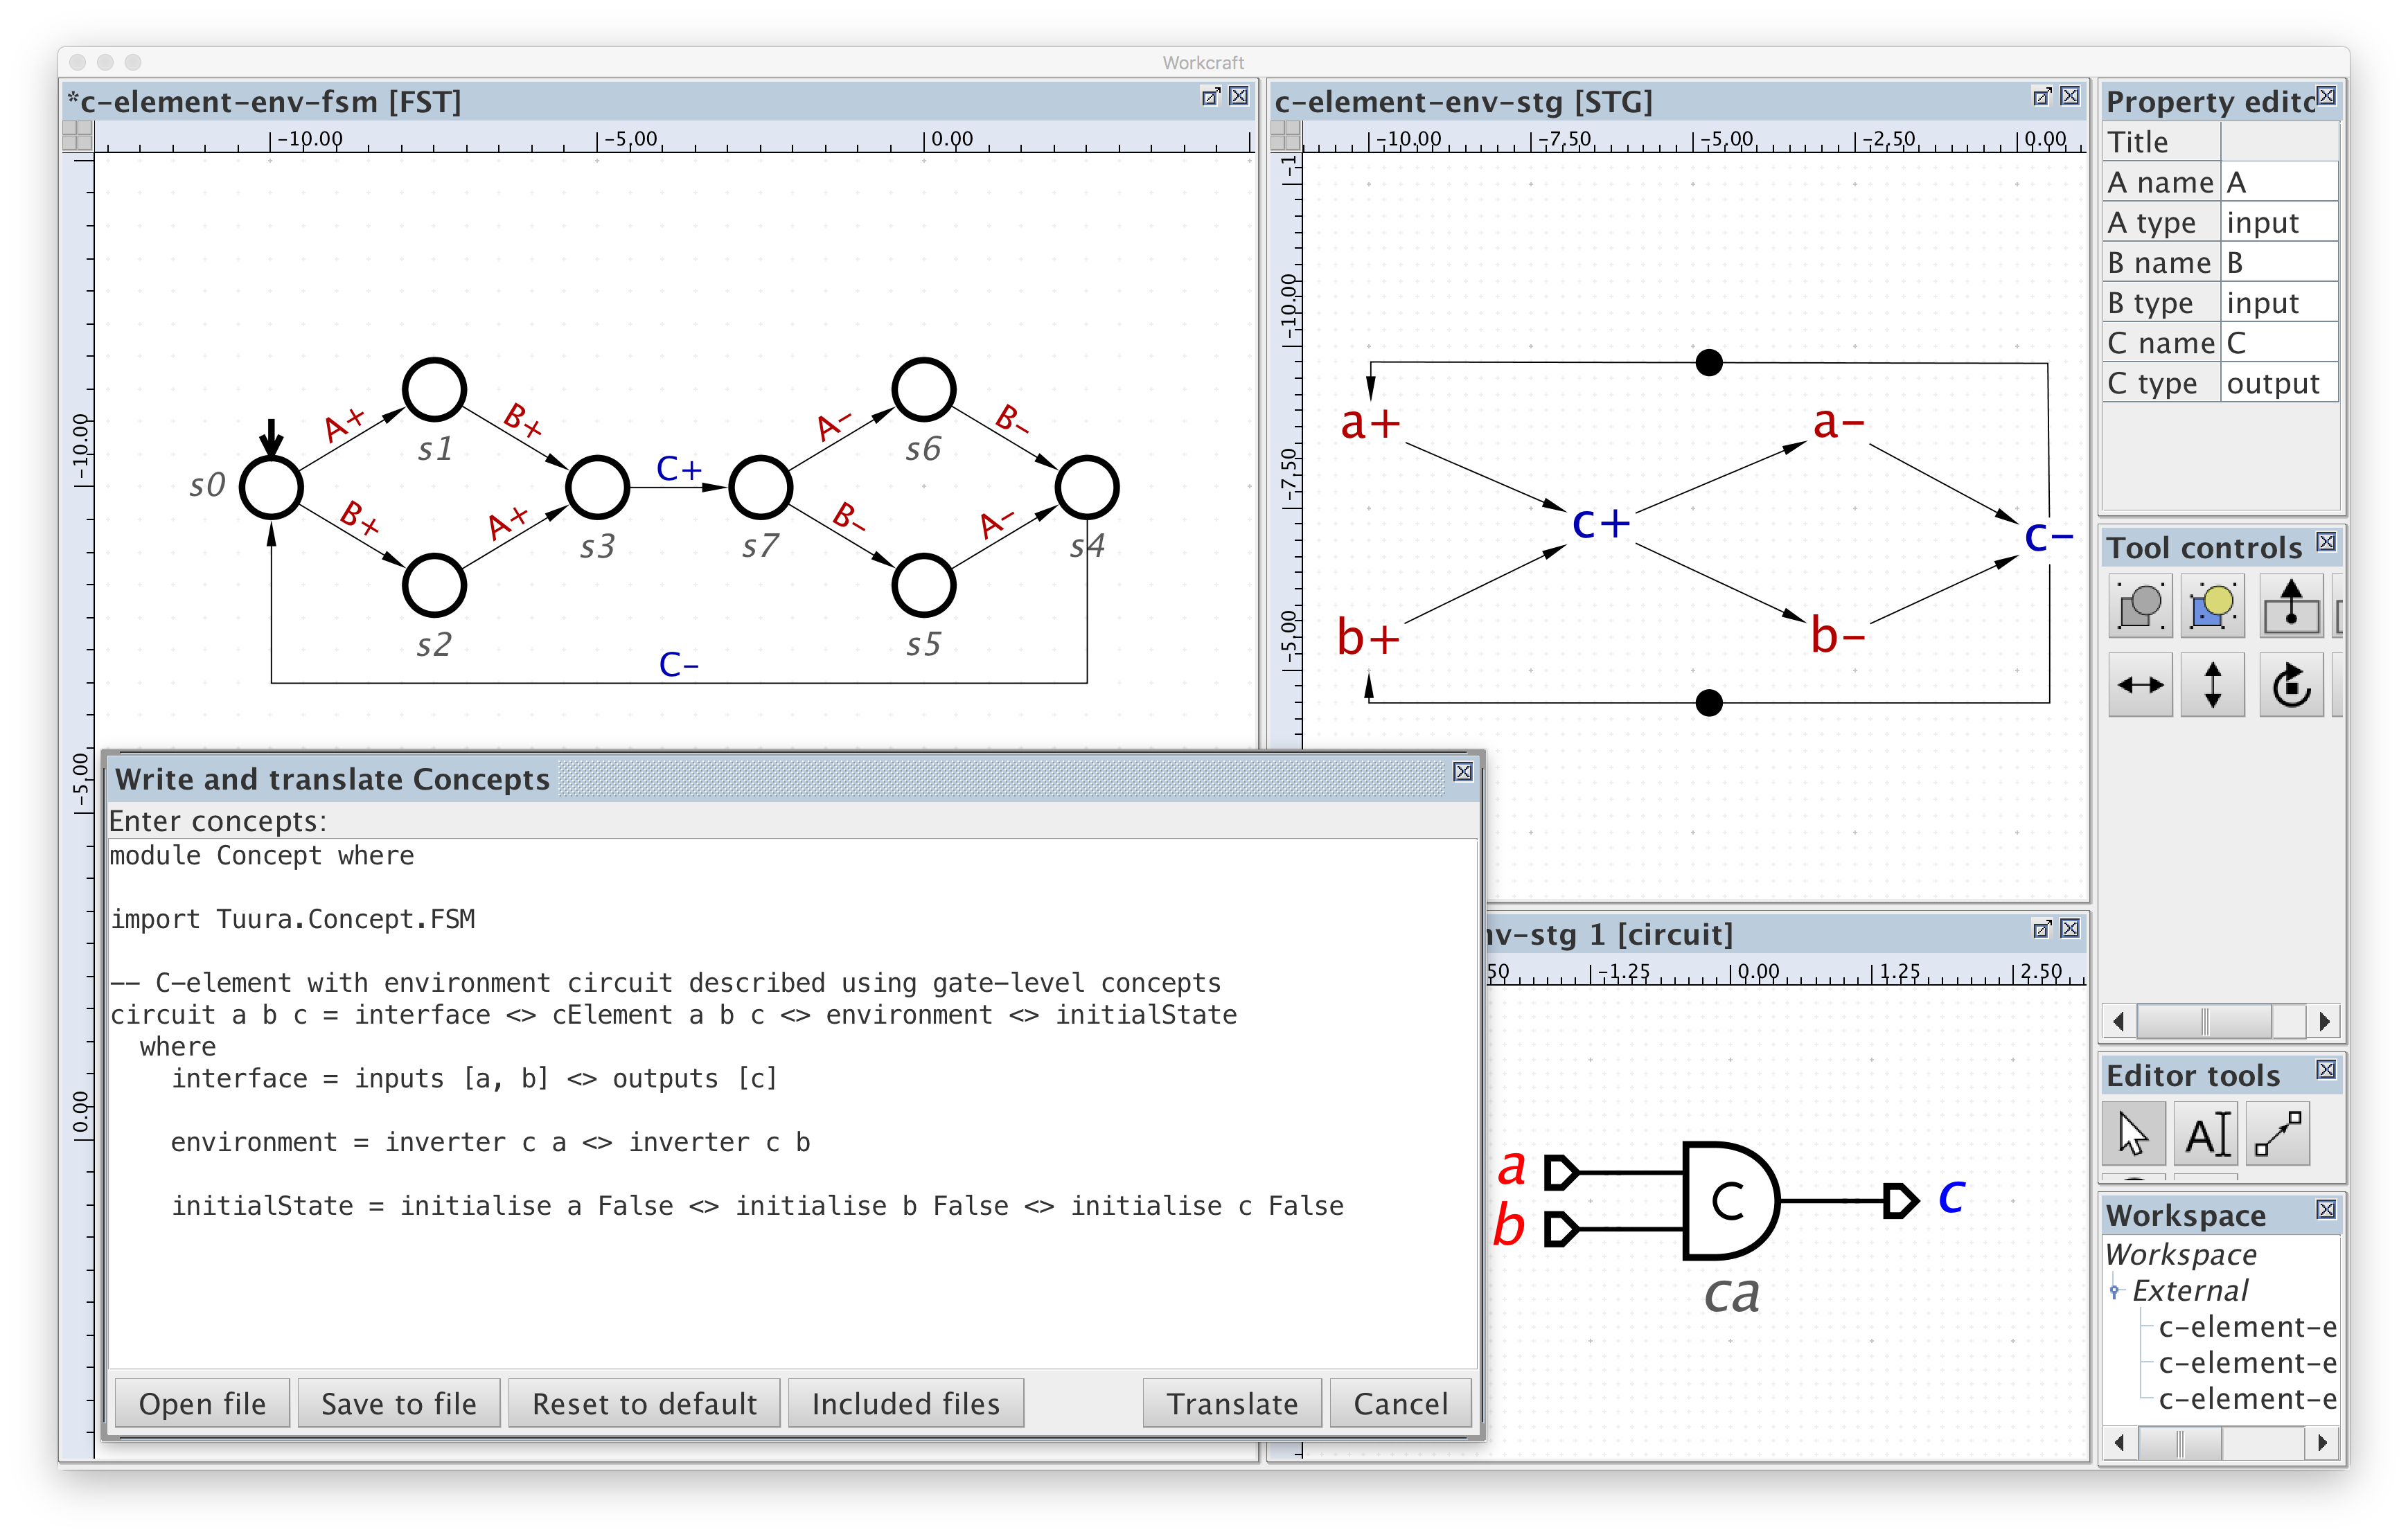
\includegraphics[scale=0.25]{images/workcraft-screenshot}
		\par\end{centering}
	\protect\caption{\label{fig:workcraft-screenshot} Example design flow in Workcraft}
\end{figure}

\noun{Plato} can be used as a command line tool, where a user can translate a concept specification, 
referencing the filepath, and importing other concept files which contain concepts used by the file to be 
translated. This will provide a user with an FSM or STG in a file format, .sg or .g respectively. These file 
formats can be used my many other tools to perform further operations on the translated models. 
 
It is also integrated into \noun{Workcraft}, an open-source tool-suite which also contains
several other back-end tools. This provides a GUI for visualising multiple modelling formalisms,
and for verification and synthesis of these models, and a visualisation of asynchronous circuits. For 
\noun{Plato} specifically, it provides the ability to directly import concept specifications as STGs, to 
write and save concept specifications, as well as open and edit existing concept files, and a window to 
select which files should be included in the translation process, in the event that the current 
specification uses concepts defined in other concept files. 

Figure~\ref{fig:workcraft-screenshot} contains an example of the design flow using \noun{Plato} from 
within \noun{Workcraft}. The bottom left contains the concepts authoring window. 
Above this is the FSM translated from 
the written concept specification, the same as seen in Figure~\ref{fig:c-element-env-fsm}. The top right 
contains the STG translated from the exact same concept specification, which is also the same as seen 
in Figure~\ref{fig:c-element-env-stg}. This STG can then be verified and synthesized using the back-end 
tools of \noun{Workcraft}, and synthesis will produce the actual gate of the C-element, as shown in the 
bottom-right of the image. 

%% Plato FSM Translation Tech Memo
%% Conclusion
\section {Conclusions \label {sec:conclusions}}

This document contains an algorithm for translating concept specifications,
describing the behaviours of the signals in an asynchronous system, to Finite
State Machines. We discuss Finite State Machines, and a form of FSMs that is 
used more specifically for the purpose of detailing the interactions between 
signals in a circuit, Finite State Transducers. We compare the differences in how
FSMs and STGs model concurrency, and the benefits that STGs provide in this 
case. We work through the algorithm with the example of a C-Element with an 
environment. Finally, we briefly discussed a design flow using this algorithm. 

This concept to FSM translation algorithm, as well as the algorithm to translate 
concepts to STGs is implemented in an open-source tool, \noun{Plato}. This tool 
also features the domain-specific language of concepts, including several built-in 
concepts providing some signal-, gate- and protocol-level concepts. This tool 
allows a user to define their own concepts, and re-use them in multiple concept 
specifications by importing the file they are in into this specification. 

\noun{Plato} provides several features to help improve the design-flow of 
asynchronous circuits, which up until know has often involved a blank page to 
start a design, unable to reuse any structures from previous designs which may 
be useful. This reuse can cause a reduced design time for asynchronous circuits, 
which in turn can make them more favourable. 

Providing the ability to translate concepts to FSMs allows a user to view the 
intricacies of a system, possible orderings of signals and how states in the 
system may be affected by signal changes, which may be desirable to an 
industrial designer, who may understand a modelling formalism such as an FSM
more than an STG. This is reccomended only for small scenarios of snippets of 
such as a design, as a larger system can make for many possible states, which 
can take a long time to translate due to state explosion. 

However, concept specifications themselves cannot be verified and synthesized 
and creating tools for this purpose is a time consuming endeavour. 
FSMs are also not the preferred model to try verification and synthesis on. 
Therefore, it is preferable to use STGs, which feature many tools for 
such operations. Thus, concepts can be freely translated to either FSMs or STGs
without editing the concepts. 

\noun{Plato} is available from~\cite{2017_plato_github}, and is also integrated 
into, and provided in the download of \noun{Workcraft}, available 
from~\cite{Workcraft_website} an open-source tool 
providing a GUI to author and translate concepts, visualise the resulting models, 
and use them with the existing tools for verification and synthesis, further 
increasing the ease and speed of design.


\bibliographystyle{unsrt}
\bibliography{publications}

\end{document}
